

\documentclass[%
 aip,
% jmp,
% bmf,
% sd,
% rsi,
cp,  % Conference Proceedings
 amsmath,amssymb,%nobibnotes,
% preprint,%
 reprint,%
%author-year,%
%author-numerical,%
]{revtex4-2}

\usepackage{graphicx}% Include figure files
\usepackage{dcolumn}% Align table columns on decimal point
\usepackage{bm}% bold math
%\usepackage[mathlines]{lineno}% Enable numbering of text and display math
%\linenumbers\relax % Commence numbering lines

\usepackage[utf8]{inputenc}
\usepackage[T1]{fontenc}
%% Loads a Times-like font. You can also load
%% {newtxtext,newtxtmath}, but not {times}, 
%% {txfonts} nor {mathtpm} as these packages
%% are obsolete and have been known to cause problems.
\usepackage{mathptmx} 
\usepackage{xcolor}
\usepackage{natbib}

% -+-+-+-+-+-+-+-+-+-+-+-+-+-+-+-+-+-+-+-+-+-+-+-+-+-+-+-+-+-+-+-+-+



\begin{document}





% Force line breaks with \\
\title{Trabalho Prático de Matemática Computacional II}

\author{Hugo Guimarães}% Write as First name Surname
\email[Corresponding author: ]{8220337@estg.ipp.pt}
\affiliation{CIICESI, ESTG, Polytechnic of Porto}

\author{João Santos} % Write as First name Surname
 \email[Corresponding author: ]{8220256@estg.ipp.pt}
\affiliation{CIICESI, ESTG, Polytechnic of Porto}
 
\author{Pedro Pinho} % Write as First name Surname
 \email[Corresponding author: ]{8220307@estg.ipp.pt}
\affiliation{CIICESI, ESTG, Polytechnic of Porto}
 
\author{Sónia Oliveira} % Write as First name Surname
 \email[Corresponding author: ]{8220114@estg.ipp.pt}
\affiliation{CIICESI, ESTG, Polytechnic of Porto}


\date{\today} % It is always \today, today, but any date may be explicitly specified


% - * - * - * - * - * - * - * - * - * - * - * - * - * - * - * - * - * - *
\begin{abstract} 
 Este relatório responde a quatro questões investigações sobre a disciplina de Engenharia de Software II para a disciplina de matemática computacional II. A primeira pergunta é saber como a taxa de cobertura dos testes evoluíram ao longo do trabalho e se a maior parte dos grupos cumpriu o critério definido no Quality Gate a cerca da taxa de cobertura dos mesmos. A segunda pergunta é se houve alguma evolução do número de linhas de código totais, e se estas estão correlacionadas com a taxa de cobertura dos testes. A terceira questão é saber quais os fatores que aumentam ou diminuem o número de testes falhados. A última questão é saber os fatores que aumentam ou diminuem o número de testes falhados
\end{abstract}



\maketitle



% - * - * - * - * - * - * - * - * - * - * - * - * - * - * - * - * - * - *
\section{INTRODUÇÃO \label{sec:intro}}
Este relatório foi criado no âmbito do trabalho prático da disciplina de Matemática computacional II, e tem como objetivo a aplicação as técnicas de análise de dados abordadas nas aulas de teóricas relativas aos conteúdos C3 C4, C5 e C6. 
Os dados analisados neste relatório são provenientes da análise de dados (reporting) de vários Projetos de Engenharia de Software II (ESII) em que cada grupo teve de efetuar recolhas semanais ao longo do desenvolvimento do projeto de ESII. Ao longo do desenvolvimento do trabalho de Matemática Computacional II, foi possível retirar conclusões interessantes, que irão ser apresentadas ao longo deste relatório, além disso, este projeto serve como forma de desenvolver a componente métrica e estatística do trabalho de Engenharia de Software II (ESII).

%Num projeto de programação, os programadores são levados a fazer várias decisões. Algumas dessas decisões podem comprometer o projeto. Por isso vamos fazer uma analise aos dados obtidos e ver o que afeta mais o projeto.%

Neste trabalho irá ser apresentado vários dados e o processo que se usou para o estudo dos mesmos:
\begin{itemize}
    \item BASE DE DADOS E METODOLOGIA – resumo dos dados e metodologia usada;
    \item RESULTADOS E DISCUSSÕES – valores obtidos da realização dos testes e discussão deles mesmos;
    \item CONCLUSÕES E TRABALHO FUTURO – conclusões sobre os dados apresentados neste documento.
\end{itemize}



%Aqui fica um exemplo de uma fórmula \textit{inline} 
 %\tau$, i.e. $v = \alpha  \left(k^2|\tau|\right)^{-1/6}$.
 
 
%No final da introdução deve incluir um parágrafo a descrever o que %será apresentado em cada secção. Por exemplo:


% - * - * - * - * - * - * - * - * - * - * - * - * - * - * - * - * - * - *
\newpage
\section{TRATAMENTO DE OUTLIERS \label{sec:simulation}  } 

Alguns dados importados possuem valores vazios (N.A) e para a resolução desses valores vazios optou-se por deixar como (N.A) quando importamos. Como foram importados os NA's, então, quando se fez os testes tentou-se sempre procurar uma opção que remova os remova.  



\section{IDENTIFICAÇÃO DAS VARIÁVEIS \label{sec:simulation}  } 

Na base de dados encontram-se 28 conjuntos de dados, que são: 
\begin{itemize}
    \item Grupo Anónimo 
    \item M1) Número de Sprint
    \item M2) Número de técnicos no projeto de ESII
    \item M3) Número de User Stories abertas
    \item M4) Número de User Stories fechadas - Entrega de SW funcional 
    \item M5) Número de pedidos de alterações abertos
    \item M6) Número de pedidos de alterações rejeitados
    \item M7) Número de pedidos de alterações aprovados 
    \item M8) Número de testes totais
    \item M9) Número de testes falhados, por sprint
    \item M10) Número de Merge Requests, por sprint
    \item M11) Número de Merge Requests falhados ou com conflitos não solucionados, por sprint
    \item M12) Número de Classes/componentes
    \item M13) Número médio de métodos por classe 
    \item M14) Cyclomatic complexity - número de itens (métodos)<10 - O plugin PMD tem regras para obtenção deste valor (CyclomaticComplexity)
    \item M15) CognitiveComplexity - número de itens (métodos) <10 - O plugin PMD tem regras para obtenção deste valor (CognitiveComplexity)
    \item M16) Class Coupling - ExcessiveImports <30; CouplingBetweenObjects<20 - Class Coupling existe quando uma classe usa outra de alguma forma. O plugin PMD tem regras para obtenção deste valor (CouplingBetweenObjects; ExcessiveImports)
    \item M17) Class Cohesion - número de itens <10 - O plugin PMD tem regras para obtenção deste valor
    \item M18) Número de Linhas de código (LOC) totais 
    \item M19) Número médio de Linhas de código (LOC) por classe
    \item M20) Número de linhas de Código duplicado totais 
    \item M21) Tempo de ciclo, em dias - tempo médio entre o primeiro commit e a versão final do sprint
    \item M22) Número de correções necessárias por tempo de ciclo
    \item M23) Número de alterações por linha de código, ou seja, ao longo dos vários commits, quantas vezes o código já foi alterado, por sprint
    \item M24) Taxa de cobertura de código nos testes unitários [0, 1], por sprint
    \item M25) Taxa de cobertura de código na fase de integração contínua [0, 1], por sprint
    \item M26) Média das notas da UC de PP de todos os técnicos do projeto
    \item M27) Média das notas da UC de ESI de todos os técnicos do projeto
\end{itemize}

\vspace{0.5cm}

\textbf{ As variáveis quantitativas discretas são: }
 M1, M2, M3, M4,M5, M6, M7 , M8, M9 e M10 \\

 
\textbf{ As variáveis quantitativas continuas são: }
M11, M12, M13, M14, M15, M16, M17, M18, M19, M20, M21, M22, M23 M24, M25, M26 e M27\\

\vspace{2cm}

\textbf{ População:  }
A população utilizada é baseadas nos alunos que entregaram recolhas vindas do projeto de ESII, e cujos resultados nos foram fornecidos para análise pelas docentes.\\



\textbf{ Amostras:  }
As amostras utilizadas diferem de questão para questão, representando, de um modo geral, um subgrupo da população cuja informação é relevante ao contexto.\\




\vspace{2cm}

\textbf{Software usados : }
\begin{itemize}
    \item R-Studio
    \item Excel
    \item Microsoft Teams
    \item Overleaf
\end{itemize}

\vspace{10pt}

\textbf{Linguagens usadas : }
\begin{itemize}
    \item R
    \item Latex
\end{itemize}

\newpage
   
% - * - * - * - * - * - * - * - * - * - * - * - * - * - * - * - * - * - *


\section{RESULTADOS E DISCUSSÕES \label{sec:Res}} 

Antes de se começar a investigação, foi preciso importar o ficheiro excel com a informação das recolhas para o RStudio, para isso, removeu-se a primeira linha do ficheiro original, para que o nome das variáveis fosse igual aos descritos na secção de identificação de variáveis, e resolveu-se alguns problemas de incoerência quanto ao carácter usado como divisor decimal. Por fim foi só exportar o ficheiro para csv, e dentro do RStudio usar o comando read-csv2 para o ler.

\vspace{10pt}

\begin{figure}[h]
    \centering
    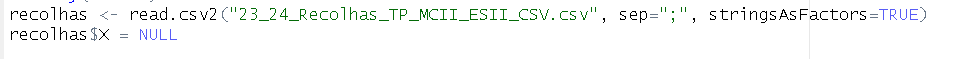
\includegraphics[width=1\linewidth]{imagens/LeituraExcel.png}
    \caption{Função usada para ler o ficheiro das recolhas}
    \label{fig:enter-label}
\end{figure}

\vspace{10pt}

\begin{figure}[h]
    \centering
    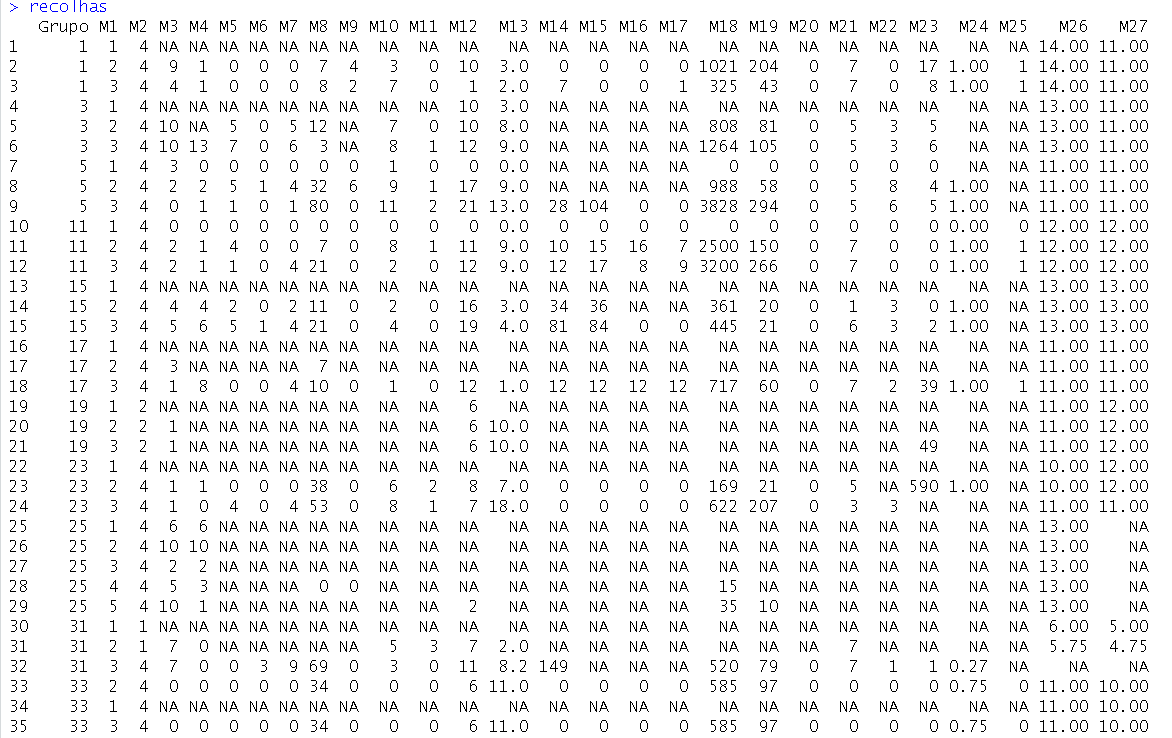
\includegraphics[width=1\linewidth]{imagens/Output_Variavel recolhas.png}
    \caption{Valor da variável data}
    \label{fig:enter-label}
\end{figure}

\newpage

\subsection{Questão de Investigação 1}
A primeira questão de investigação trata-se de \textbf{saber a evolução da taxa de cobertura dos testes e saber se os grupos cumpriram o critério definido no Quality Gate dos trabalhos de Engenharia de Software II para a taxa de cobertura admissível dos mesmos}. Para o estudo dessa métrica, foi analisado o ficheiro Excel e verificou-se que dever-se-ia usar a variável M24 (taxa de cobertura de código nos testes unitários [0, 1], por sprint). Após essa verificação percebeu-se que deveria de ser um teste de proporção, pois serão analisadas as taxas de cobertura da segunda e da quarta semana, e este teste permite-nos saber se existiu mudanças significativas entre as duas. Para a realização de todos os testes optou-se por um nível de significância de 5\%.

\vspace{0.5cm}

Primeiramente, removeu-se todas as linhas com valores omissos (NA), depois, selecionou-se as colunas relevantes (M1 e M24) para a segunda e a quarta semana. Após a seleção das colunas resolveu-se fazer o summary para cada semana, o resultado desse comando pode ser visualizado na Tabela \ref{Summary_Semana2} e na Tabela \ref{Summary_Semana4}, para além do summary, também se criou um Boxplot para poder haver um apoio visual ao tirar conclusões, esse gráfico pode ser visto na Figura \ref{Boxplot_Semana2_4}

\begin{table}[!h]
    \centering
    \caption{Medidas de Localização dos dados da taxa de cobertura da segunda semana}
    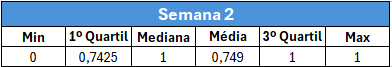
\includegraphics[width=8cm]{imagens/questao1/tabelaSummarySemana2.png}
    \label{Summary_Semana2}
\end{table}

\begin{table}[!h]
    \centering
    \caption{Medidas de Localização dos dados da taxa de cobertura da quarta semana}
    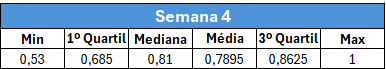
\includegraphics[width=8cm]{imagens/questao1/tabelaSummarySemana4.png}
    \label{Summary_Semana4}
\end{table}

\begin{figure}[!h]
    \centering
    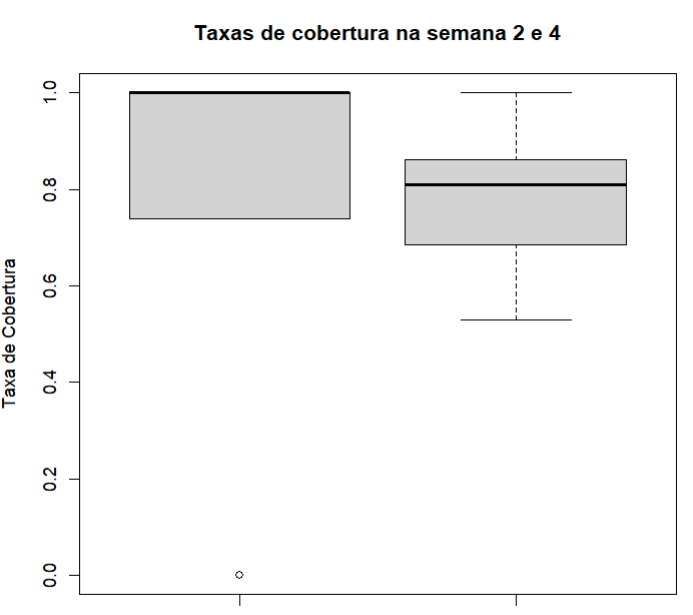
\includegraphics[width=8cm]{imagens/questao1/Boxplot_Semana2_4.png}
    \caption{Boxplot da distribuição da taxa de cobertura da semana 2 (à esquerda) e da semana 4 (à direita)}
    \label{Boxplot_Semana2_4}
\end{figure}

Com essa informação, conseguiu-se observar que na segunda semana a mediana está com o valor 1, isso significa que metade das pessoas têm uma taxa de cobertura de 100\%. Já na quarta semana consegue-se observar que a taxa de cobertura diminuiu, logo, a taxa de cobertura dos testes da segunda semana é significativamente maior do que na quarta semana, provavelmente, isso deve-se pois na quarta semana existe muito mais código para ser testado. No entanto, estas são as medidas de localização das amostras e não da população, não sendo suficientes para tirar conclusões.


Antes da realização do t-test, primeiro precisa-se que um conjunto de pressupostos sejam cumpridos, para isso, realizou-se um teste de variâncias, pois é preciso especificar no teste se as variâncias são iguais ou não, já que estamos a fazer um teste com duas variáveis, e um teste de normalidade, pois para poder fazer um t-test, precisa-se que os dados sigam uma distribuição normal, e como temos menos que trinta amostras, não podemos assumi-la.
\[ H0: \sigma^2_{semana2} = \sigma^2_{semana4}  \hspace{1cm} vs: \hspace{1cm} H1: \sigma^2_{semana2} \ne \sigma^2_{semana4} \]
\begin{figure}[h]
    \centering
    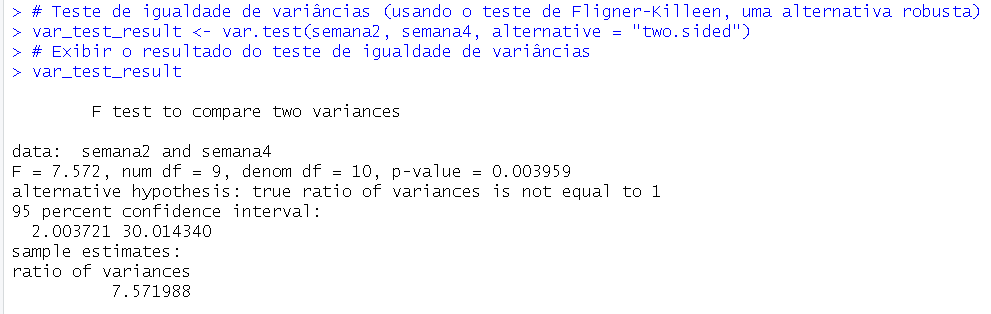
\includegraphics[width=15cm]{imagens/questao1/Output_variancia.png}
    \caption{Output do teste da variância das taxas de cobertura dos testes da segunda e da quarta semana}
    \label{Output_Variancia}
\end{figure}

Na Figura \ref{Output_Variancia} verifica-se que o p-value do teste de variâncias(0.004) é menor que que o nível de significância estipulado de 5\%, assim, rejeitando a hipótese nula, isto quer dizer que existem evidências estatísticas que as variâncias das taxas de cobertura das duas semanas são diferentes. Com esta informação, sabemos que, se um t-test for usado, precisa-se de especificar que as variâncias não são iguais


\begin{center}
    H0: A taxa de cobertura da semana i segue uma distribuição normal
    \newline
    vs:
    \newline
    H1: A taxa de cobertura da semana i não segue uma distribuição normal
    \newline
\end{center}
$i \in \{2, 3, 4\}$

\begin{figure}[!h]
    \centering
    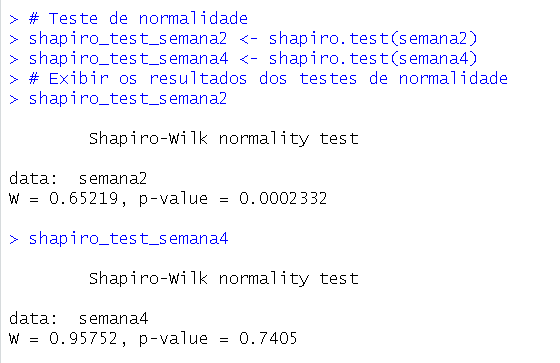
\includegraphics[width=10cm]{imagens/questao1/Shapiro_Q1.png}
    \caption{Output do teste da normalidade dos dados das taxas de cobertura dos testes da segunda e da quarta semana}
    \label{Output_Shapiro_Q1}
\end{figure}

 Na Figura \ref{Output_Shapiro_Q1} verifica-se que na segunda semana o p-value(0.002) é menor que o nível de significância estipulado de 5\%, assim a hipótese nula é rejeitada, isto quer dizer que existem evidências estatísticas que os dados sobre as taxas de cobertura da segunda semana não seguem uma distribuição normal, portanto, já não se pode usar o t-test, pois os pressupostos do mesmo não são cumpridos, vai ter de usar um teste não paramétrico para o substituir, pois estes não precisam de cumprir tantos pressupostos.
 Para substituir o t-test, optou-se por usar um teste de Wilcoxon, pois é um teste não paramétrico bom para comparar duas amostras independentes, mas ao contrário do t-test que testava as médias, este testa as medianas.

\vspace{10pt}



\begin{figure}[h]
    \centering
    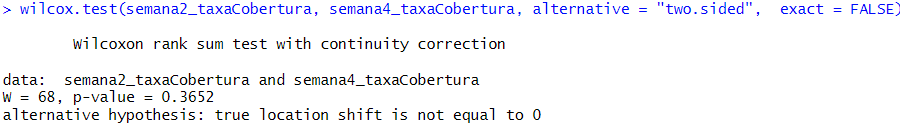
\includegraphics[width=13cm]{imagens/questao1/wilcoxon_Teste.png}
    \caption{Output do teste de Wilcoxon sobre os dados das taxas de cobertura dos testes da segunda e da quarta semana}
    \label{wilcoxon_Test}
\end{figure}

\[ H0: {\eta}_{semana2} = {\eta}_{semana4}  \hspace{1cm} vs: \hspace{1cm} h1: {\eta}_{semana2} \ne {\eta}_{semana4} \] % \eta é a variancia

 
Na Figura \ref{wilcoxon_Test}, verifica-se que o p-value dos teste de Wilcoxon(0.37) é maior que o nível de significância estipulado de 5\%, assim a hipótese nula não é rejeitada, concluindo-se que não existem evidencias estatísticas que as medianas das taxas de cobertura da segunda semana e da quarta semana sejam diferentes.
Como o a hipótese nula não foi rejeitada, então não será necessário fazer um teste unilateral para saber qual a semana com maior e menor mediana.


Por fim, para a realização dos testes de proporção foi usado um cálculo para somar todos elementos cuja taxa de cobertura fosse superior a 80\%, esse valor é definido no Quality Gate para os trabalhos da disciplina de Engenharia de Software II.

\begin{figure}[h]
    \centering
    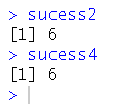
\includegraphics[width=4cm]{imagens/numero_casos.png}
    \caption{Número de casos onde a taxa de cobertura é maior que 80\% nas duas semanas}
    \label{num_casos}
\end{figure}

\begin{figure}[!h]
    \centering
    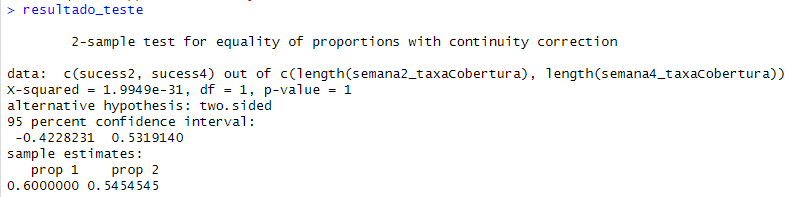
\includegraphics[width=16cm]{imagens/questao1/Output_teste_proporcao.png}
    \caption{Output do testes de proporção sobre os dados das taxas de cobertura dos testes da segunda e da quarta semana}
    \label{OutputProporcao}
\end{figure}

\hfill \break
\begin{center}
    H0: $P_1 = P_2$
    \newline
    vs:
    \newline
    H1: $P_1 \ne P_2$
    \newline
\end{center}
\hfill \break
$p_1$ - grupos com taxas de cobertura superiores a 80\% na primeira semana\\
$P_2$ - grupos com taxas de cobertura superiores a 80\% na segunda semana\\



Observou-se na Figura \ref{num_casos} que, tanto na segunda semana, como na quarta semana houveram 6 casos onde as taxas de cobertura foram maiores ou iguais a 80\%. Com o teste de proporção observa-se que na segunda semana tem uma proporção de 0.60 e já na quarta semana tem uma proporção de 0.55, e que existe um intervalo de confiança de 95\% para a diferença nas proporções que varia entre aproximadamente -0.42 a 0.53. Algo importante a destacar, é que embora a segunda e a quarta semana tenham o mesmo número de casos onde a taxa de cobertura é maior que 80\%, as proporções de ambas são diferentes, isto deve-se ao facto que as ficaram com tamanhos diferentes depois que os valores omissos foram descartados. A segunda semana tem 10 valores, já a quarta semana tem 11 valores.

No output da Figura  \ref{num_casos} pode-se ver que o p-value (1.00) é maior que o nível de significância estabelecido de 5\%, não rejeitando a hipótese nula, mostrando que existem evidências estatísticas que a proporção da primeira semana é igual à proporção da segunda semana

\vspace{1cm}

Para finalizar, para verificar se os grupos atenderam à métrica definida no Quality Gate para os trabalhos de Engenharia de Software II de 80\%, foi feito um teste de Wilcoxon onde se vai comprar se a mediana das taxas de cobertura dos testes da quarta semana foi inferior a 80\%.

\[ H0: \eta_{semana2} = 80\%  \hspace{1cm} vs: \hspace{1cm} H1: \eta_{semana2} < 80\% \]

\begin{figure}[!h]
    \centering
    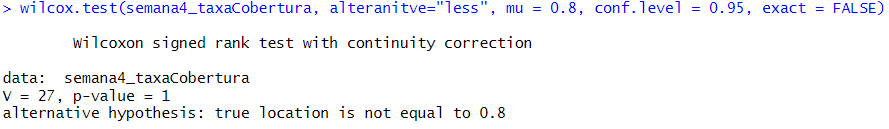
\includegraphics[width=0.9\linewidth]{imagens//questao1/testeUmaVariavel.png}
    \caption{Teste de Wilcoxon para saber se os grupos respeitaram o Quality Gate para a taxa de cobertura dos testes}
    \label{fig:QualityGateCheck}
\end{figure}

A partir da Figura \ref{fig:QualityGateCheck} consegue-se ver que o p-value (1.00) é maior que o nível de significância estabelecido de 5\%, logo a hipótese nula não é rejeitada, havendo evidências estatísticas que a taxa de cobertura dos testes da quarta semana é igual a 80\%

\vspace{1cm}

\textbf{Conclusão:} Com os testes realizados, provou-se que  não existe evolução significativa na taxa de cobertura dos testes entre a segunda e a quarta semana, e que a maior parte dos alunos respeitou a métrica defendia no Quality Gate de Engenharia de Software II, onde se deve ter uma taxa de cobertura dos testes de no mínimo 80\%

\newpage




\subsection{Questão de Investigação 2}
Na primeira questão, após serem analisados os dados das taxas de cobertura dos testes da segunda e da quarta semana, observou-se que segundo esses dados a taxa de cobertura da segunda para a quarta semana diminuiu, e afirmou-se se que provavelmente isso aconteceu pois havia mais código para testar, portanto para esta questão de investigação vai-se \textbf{verificar se houve um aumento no número de linhas de código totais (M18), e se elas estão correlacionadas com a taxa de cobertura dos testes (M24)}

Para verificar se houve um aumento no número de linhas de código totais, começou-se por separar o número de linhas de código escritas na segunda, terceira e quarta semana e escreveu-se um sumário para cada uma e um boxplot para estudar os dados das três amostras. Não serão estudadas o número de linhas de código totais da primeira semana, pois, como ainda não era preciso escrever código para o trabalho de Engenharia de Software II, a maior parte dos grupos deixou esse campo em branco.

\begin{table}[!h]
    \centering
    \caption{Medidas de localização do número de linhas de código totais da segunda semana}
    \label{fig:sumarryLinhasSemana2}
    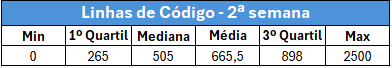
\includegraphics[width=0.5\linewidth]{imagens//questao2/sumarryLinhasSemana2.png}
    \label{fig:sumarryLinhasSemana2}
\end{table}

\begin{table}[!h]
    \centering
    \caption{Medidas de localização do número de linhas de código totais da terceira semana}
    \label{fig:sumarryLinhasSemana3}
    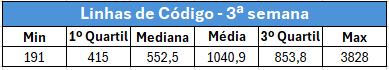
\includegraphics[width=0.5\linewidth]{imagens//questao2/sumarryLinhasSemana3.png}
    \label{fig:sumarryLinhasSemana3}
\end{table}

\begin{table}[!h]
    \centering
    \caption{Medidas de localização do número de linhas de código totais da quarta semana}
    \label{fig:sumarryLinhasSemana4}
    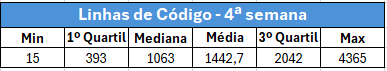
\includegraphics[width=0.5\linewidth]{imagens//questao2/sumarryLinhasSemana4.png}
\end{table}

\begin{figure}[!h]
    \centering
    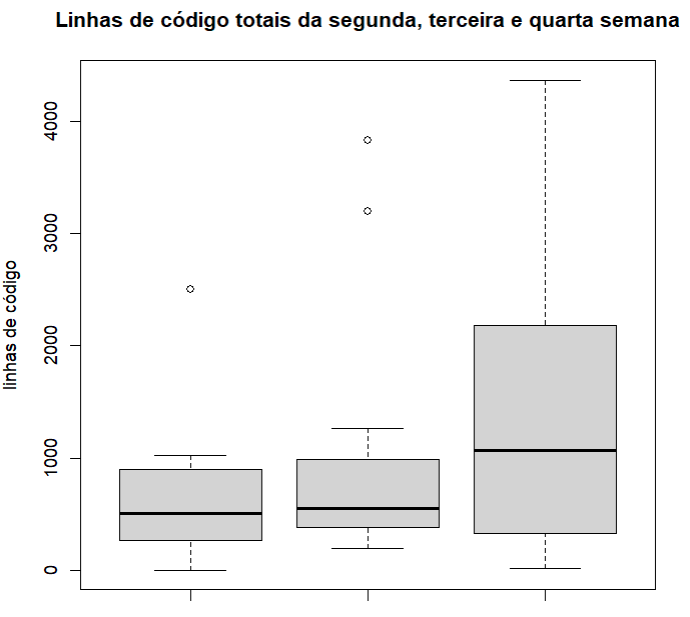
\includegraphics[width=0.5\linewidth]{imagens//questao2/boxplotDas3Semanas.png}
    \caption{BoxPlot do número de linhas de código totais da 2ª, 3ª e 4ª semana}
    \label{fig:BoxPlotDas3Semanas}
\end{figure}

Como dá para ver pelos sumários das Tabelas  \ref{fig:sumarryLinhasSemana2},  \ref{fig:sumarryLinhasSemana3}, \ref{fig:sumarryLinhasSemana4}, e sobretudo no boxplot da Figura \ref{fig:BoxPlotDas3Semanas}, consegue-se ver que consoante as semanas passavam, o número de linhas de código aumentavam.

Ao analisar o sumário do número de linhas de código totais na segunda semana (Tabela \ref{fig:sumarryLinhasSemana2}), percebe-se que o primeiro quartil ($Q_1$) é de 265.0, que pelo menos 25\% dos grupos tiveram pelo menos 265 linhas de código totais o segundo quartil ($Q_2$, ou mediana) é de 505.0, que 50\% dos grupos tiveram pelo menos 505 linhas de código totais, e o terceiro quartil ($Q_3$) atinge 898.0, que pelo menos 75\% dos grupos tiveram pelo menos 898 linhas de código totais. Já na terceira semana (Tabela \ref{fig:sumarryLinhasSemana3}), consegue-se ver que houve um aumento significativo nos quartis, com $Q_1=415.0$, $Q_2=552.5$, e $Q_3=853.8$. No final, na quarta semana (Tabela \ref{fig:sumarryLinhasSemana4}), os valores continuaram a crescer com os quartis $Q_1=393.5$, $Q_2=1063.0$, e $Q_3=2042.0$.

Estas observações são confirmadas visualmente com o boxplot da Figura \ref {fig:BoxPlotDas3Semanas}, onde é possível perceber uma tendência no aumento no número de linhas de código ao longo das semanas, podendo ver isso através da linha mais escura no maio das caixas, que é a mediana, que vai aumentando consoante as semanas passavam. Este comportamento ascendente sugere que o desenvolvimento de código tornou-se mais extenso à medida que o projeto avançava, possibilitando uma correlação entre o tempo e o número de linhas de código. Outro ponto que também é possível ver a partir do boxplot, é que a caixa da terceira semana é muito maior do que a da segunda e terceira semana, isso significa que existe uma maior dispersão nos dados da quarta semana, que tem uma amplitude inter-quartil maior

No entanto, estes dados refletem apenas as medidas de localização das amostras, não representado os valores reais da população, portanto vai ter de se fazer mais testes para verificar se houve mesmo um aumento do número de linhas de código totais. Para fazer esse estudo, decidiu-se fazer um teste de ANOVA, pois, ele permite comparar as médias populacionais de mais de dois grupos, no entanto para poder usar esse teste é preciso saber se as amostras seguem uma distribuição normal, para isso vai-se fazer o teste de Shapiro-Wilk para as três amostras.

\begin{figure}[!h]
    \centering
    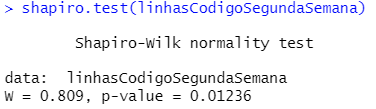
\includegraphics[width=0.6\linewidth]{imagens//questao2/testeShapiroLinhasSegundaSemana.png}
    \caption{Teste de normalidade aos dados do número de  linhas de código da segunda semana}
    \label{fig:shapiroTesteSemana2Linhas}
\end{figure}

\begin{figure}[!h]
    \centering
    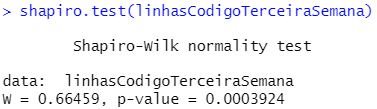
\includegraphics[width=0.6\linewidth]{imagens//questao2/testeShapiroLinhasTerceiraSemana.png}
    \caption{Teste de normalidade aos dados das linhas de código totais da terceira semana}
    \label{fig:shapiroTesteSemana3Linhas}
\end{figure}

 \begin{figure}[!h]
     \centering
     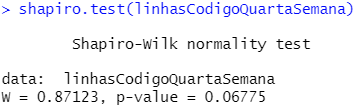
\includegraphics[width=0.6\linewidth]{imagens//questao2/testeShapiroLinhasQuartaSemana.png}
     \caption{Teste de normalidade aos dados do número de linhas de código totais da quarta semana}
     \label{fig:shapiroTesteSemana4Linhas}
 \end{figure}


\begin{center}
    H0: O número de linhas de código totais da semana i seguem uma distribuição normal
    \newline
    vs:
    \newline
    H1: O número de linhas de código totais da semana i não seguem uma distribuição normal
    
\end{center}
$i \in \{2, 3, 4\}$ \\


 Nas Figuras \ref{fig:shapiroTesteSemana2Linhas} e \ref{fig:shapiroTesteSemana3Linhas}, consegue-se ver que o p-value (0.01236 para a segunda semana e 0.0003924 para a terceira semana) é menor que o nível de significância estabelecido de 5\%, rejeitando a hipótese nula, existindo evidências estatísticas que os dados sobre o número de linhas de código totais da segunda e terceira semana não seguem uma distribuição normal. No entanto, na Figura \ref{fig:shapiroTesteSemana4Linhas}, o p-value (0.06775) é maior que o nível de significância estabelecido de 5\%, não rejeitando a hipótese nula, existindo evidências estatísticas que os dados sobre o número de linhas de código da quarta semana seguem uma distribuição normal.
 Como apenas os dados da quarta semana seguem uma distribuição normal, já não dá para usar um teste de ANOVA, assim, vai ter de ser substituído por um teste não paramétrico, sendo o teste escolhido o de Kruskal-Wallis, visto que as amostras são independentes, nele é testado a igualdade das medianas de todos os grupos, ao contrário do teste de ANOVA que testava as médias. Caso as amostras fossem emparelhadas, ter-se-ia de usar um teste de Friedman.

\[ H0: {\eta}_{semana2} = {\eta}_{semana3} = {\eta}_{semana4}  \hspace{1cm} vs: \hspace{1cm} h1: {\eta}_{semana2} \ne {\eta}_{semana3} \ne {\eta}_{semana4} \]

\begin{figure}[!h]
    \centering
    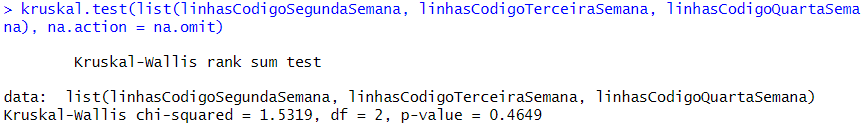
\includegraphics[width=0.9\linewidth]{imagens//questao2/testeKruskaWallis.png}
    \caption{ Teste de Kruskall-Wallis para comparar as medianas da segunda, terceira e quarta semana}
    \label{fig:kruskalWallisTestPergunta2}
\end{figure}

A partir do output da Figura \ref{fig:kruskalWallisTestPergunta2}, consegue-se ver que o p-value (0.4649) é maior que o nível de significância estabelecido de 5\%, logo a hipótese nula não é rejeitada, verificando-se que ao contrário do que foi visto na análise análise das amostras, existem evidências estatísticas que as medianas do número de linhas de código totais das três semanas são estatisticamente iguais.

%---------------------------------------daria para fazer uma nova pergunta com o que vem para a frente
Após se verificar que não houve aumento significativo no número de linhas de código totais, vai-se confirmar se estas correlacionam com a taxa de cobertura dos testes, e provar se a afirmação da primeira pergunta é válida.

Para poder estudar a validade dessa afirmação, vai ter de se fazer um teste de correlação para saber se os dados sobre o número de linhas de código totais estão correlacionados com os dados da taxa de cobertura dos testes, mas antes é preciso fazer um teste de normalidade às duas amostras para saber se se vai usar um teste de correlação de Pearson ou um teste de correlação de Spearman.

Nos dados a cerca do número de linhas de código totais e da taxa de cobertura dos testes, foram ignorados os dados da primeira semana, pois nessa altura ainda não era preciso escrever código, havendo assim muito pouca informação, e a escassa informação que tem pode não ser credível.


\begin{figure}
    \centering
    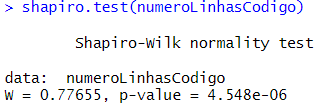
\includegraphics[width=0.5\linewidth]{imagens//questao2/shapiroTestLinhasDeCodigoParaCorrelacao.png}
    \caption{Teste de normalidade de Shapiro-Wilk para os dados sobre o numero de linhas de código totais}
    \label{fig:ShairoTestLinhasParaCorrelacao}
\end{figure}
\begin{figure}
    \centering
    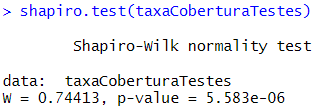
\includegraphics[width=0.5\linewidth]{imagens//questao2/ShapiroTestTaxaCoberturaParaCorrelacao.png}
    \caption{Teste de normalidade de Shapiro-Wilk para os dados sobre a taxa de cobertura dos testes}
    \label{fig:ShairoTestTaxaCoverturaParaCorrelacao}
\end{figure}

\begin{center}
    H0: O número de linhas de código totais seguem uma distribuição normal
    \newline
    vs:
    \newline
    H1:O número de linhas de código totais não seguem uma distribuição normal
    \newline
\end{center}


\begin{center}
    H0: A taxa de cobertura dos testes seguem uma distribuição normal
    \newline
    vs:
    \newline
    H1:A taxa de cobertura dos testes não seguem uma distribuição normal
    \newline
\end{center}

Como dá para ver nas Figuras \ref{fig:ShairoTestLinhasParaCorrelacao} e \ref{fig:ShairoTestTaxaCoverturaParaCorrelacao}, os p-values dos dois testes ($4.548 * 10^{-6}$ e $5.583 * 10^{-6}$) são menores que o nível de significância estabelecido de 5\%, rejeitando a hipótese nula, comprovando que existem evidências estatísticas que os dados do número de linhas de código totais e da taxa de cobertura dos testes não seguem uma distribuição normal, assim será preciso usar um teste de correlação de Spearman, pois este é uma alternativa não paramétrica ao teste de Pearson, que precisa que os dados sigam uma distribuição normal.

\begin{figure}[!h]
    \centering
    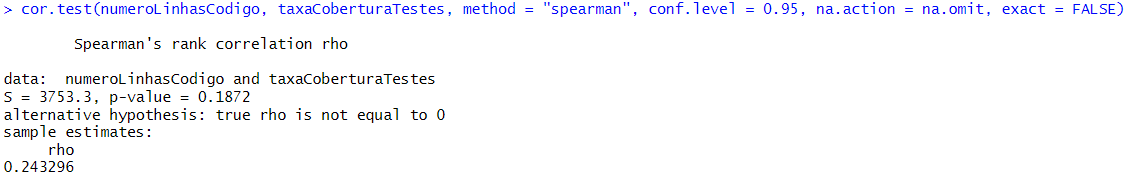
\includegraphics[width=1\linewidth]{imagens//questao2/pergunta2TesteCorrelacaoSpearman.png}
    \caption{Teste de correlação de Spearman para os dados do número de linhas de código totais e para a taxa de cobertura dos testes}
    \label{fig:TesteCorrelacaoSpearmanPergunta2}
\end{figure}



\begin{center}
H0: Coeficiente de correlação é igual a 0 \\ vs: \\ H1: Coeficiente de correlação é diferente a 0
\end{center}

A partir do output da Figura \ref{fig:TesteCorrelacaoSpearmanPergunta2} é possível verificar que o p-value (0.1872) é menor que o nível de significância estabelecido de 5\%, não rejeitando a hipótese nula, existindo evidências estatísticas que o coeficiente de correlação é igual a 0.
O coeficiente de correlação de Spearman, denominado por $\rho $ (rho), é um número que varia entre -1 e 1. Quanto mais próximo dos extremos (-1 ou 1), maior é a força da correlação. Já os valores próximos de 0 implicam em correlações mais fracas ou inexistentes. No output apresentado, é possível ver que o coeficiente de correlação (0.243296) está muito próximo de zero.

Outra forma de ver a correlação entre os dados é através de um gráfico de dispersão, assim é possível identificar padrões e tendências nos mesmos, servindo como guia visual entre a relação entre as duas variáveis.
Na Figura \ref{fig:ScatterPlotPergunta2}, é apresentado um gráfico de dispersão que representa os pontos correspondentes ao número de linhas de código totais no eixo x, e à taxa de cobertura dos testes no eixo y, onde cada ponto no gráfico representa uma observação. A inclinação geral da dispersão dos pontos pode indicar a direção da relação entre as variáveis: se os pontos estão inclinados para cima, sugere uma correlação positiva, enquanto uma inclinação para baixo indica uma correlação negativa.

A adição da linha de regressão linear, representada  vermelho, ajuda a destacar a tendência geral dos dados, mesmo que, segundo o resultado do teste de correlação de Spearman, não tenha sido encontrada uma correlação significativa entre as variáveis.

 \begin{figure}[!h]
     \centering
     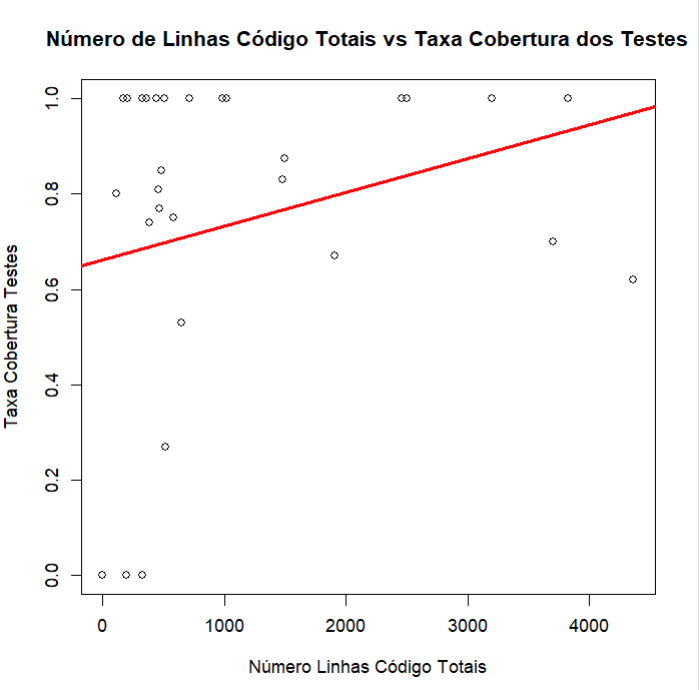
\includegraphics[width=0.4\linewidth]{imagens//questao2/scatterPlotCorrelacaoPergunta2.png}
     \caption{Gráfico de dispersão dos dados do número linhas de código totais com a taxa de cobertura dos testes}
     \label{fig:ScatterPlotPergunta2}
 \end{figure}
 
\vspace{2cm}

 \textbf{Conclusão:} Com os testes realizados, provou-se que para além de não ter havido uma evolução significativa no número de linhas de código totais no decorrer do projeto de Engenharia de Software II, também se provou que a afirmação feita na primeira pergunta não tem validade, os dados sobre o número de linhas de código totais e a taxa de cobertura dos testes não estão correlacionados


\newpage


\subsection{Questão de Investigação 3}
A terceira questão de investigação trata-se de \textbf{saber os fatores que aumentam ou diminuem o número de testes falhados (M9)}, para isso, será preciso montar um modelo de regressão linear para saber quais as variáveis que influenciam o valor da variável $M9$.


Para montar o modelo de regressão linear, primeiramente realizou-se uma matriz de correlações com todas as variáveis das recolhas, com essa matriz, é possível visualizar quais variáveis têm uma maior correlação com quais variáveis. Como existem muitas variáveis onde os dados não seguem uma distribuição normal, decidiu-se usar o método de \textit{Spearman} para a montagem da matriz

\begin{figure}[!h]
    \centering
    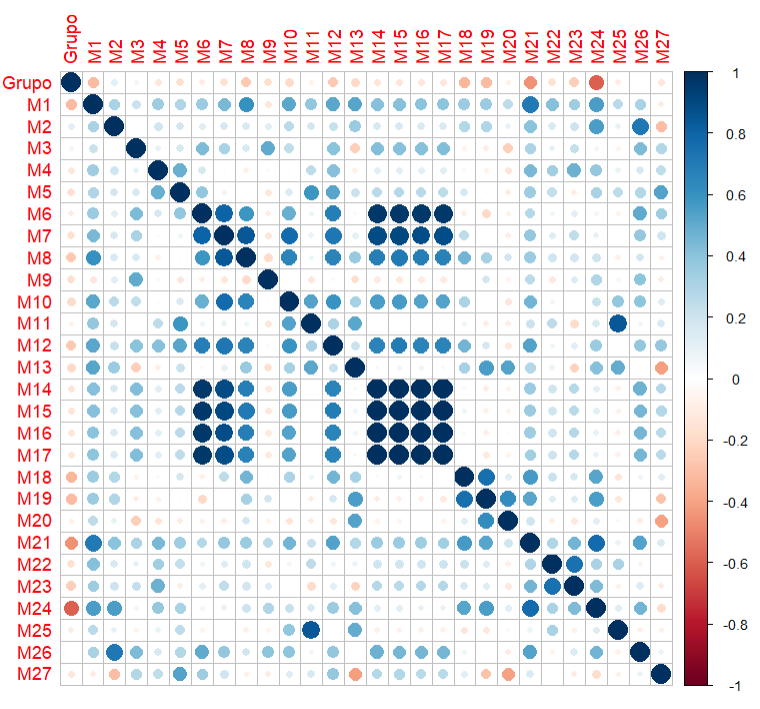
\includegraphics[width=10cm]{imagens/questao3/questao3_matriz de correlacoes.png}
    \caption{Matriz de correlações de todos os dados recolhidos}
    \label{questao3matrizDeCorrelacoes}
\end{figure}

Como dá para ver na Figura \ref{questao3matrizDeCorrelacoes}, as correlações para a variável M9, o número de testes falhados, são bastante fracas. O nível de correlações consegue ser visualizado a partir da cor, onde, quanto mais clara é a cor indica valores próximos de zero ou correlações mais fracas, enquanto que cores mais escuras indicam valores mais extremos ou correlações mais fortes.


Mesmo com correlações bastante fracas, vai-se tentar montar um modelo de regressão linear com as variáveis $M03$, $M04$, $M05$ e $M22$, pois, dentro de todas as correlações vistas na coluna $M09$ na matriz de correlações, estas são as que têm uma maior correlação.

\begin{itemize}
    \item $M03$ - Número de User Stories abertas 
    \item $M04$ - Número de User Stories fechadas 
    \item $M05$ - Número de pedidos de alterações abertos
    \item $M22$ - Número de correções necessárias por tempo de ciclo
\end{itemize}

Como a questão em estudo trata-se de fatores que aumentam e diminuem o número de testes, a melhor forma para o analisar seria através de um modelo de regressão linear, neste caso em questão, uma regressão linear múltipla, onde numa primeira etapa foi montado da seguinte forma: a variável $M09$ é a variável dependente, e as variáveis $M03$, $M04$, $M05$ e $M22$ são as variáveis independentes.\\

Modelo de regressão linear: \[ M09 = a0 + a1*M03 + a2*M04 + a3*M05 + a4*M22 + \varepsilon\]

\begin{figure}[!h]
    \centering
    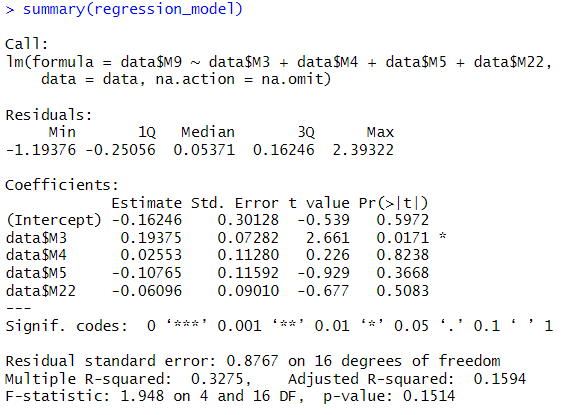
\includegraphics[width=11cm]{imagens/questao3/questao3PrimeiraregressaoLinear.png}
    \caption{Primeiro modelo de correlação}
    \label{questao3OutputCorrelacao1}
\end{figure}

\vspace{0.2cm}

Na Figura \ref{questao3OutputCorrelacao1} é possível fazer um teste global para saber se o modelo é válido, para isso,  tem que se olhar para a secção F-statistic e verificar se o p-value de lá é menor que o nível de significância estabelecido, como o p-value (0.1514) é maior que o nível de significância estabelecido, isso significa que a hipótese nula não é rejeitada, havendo evidências estatísticas que as variáveis independentes não têm um efeito significativo sobre a variável dependente

Teste Global: 
\begin{center}
        $H0:  a_{1} = a_{2} = ... = a_{i} = 0 $\hspace{0.5cm}
    vs. \hspace{0.5cm}
   $ H1:$  existe pelo menor um i, onde $a_{i} \ne 0$
\end{center}



Para encontrar um modelo de regressão válido, ter-se-ia que descartar variáveis dependentes e executar de novo o modelo de regressão linear sucessivamente até encontrar o modelo mais adequado, para fazer isso utilizou-se uma técnica de seleção de variáveis denominada de \textit{stepwise}.

O método \textit{stepwise} tenta automatizar o processo de seleção das variáveis mais otimizadas para o modelo de regressão linear, considerando critérios como AIC (Akaike Information Criterion) ou BIC (Bayesian Information Criterion). Dessa forma, ao aplicar o \textit{stepwise} o modelo será ajustado consecutivamente, adicionando ou removendo variáveis até encontrar um modelo adequado.

\begin{figure}[!h]
    \centering
    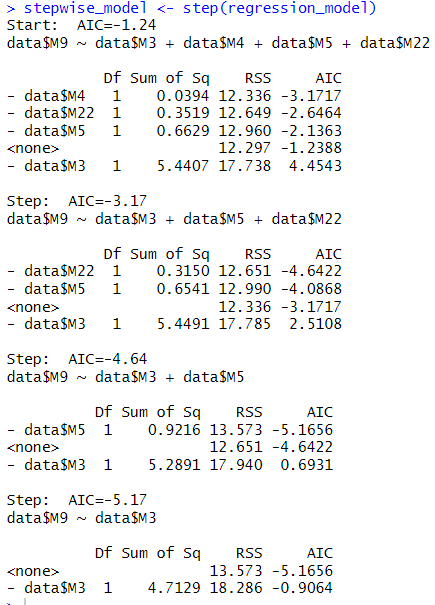
\includegraphics[width=0.5\linewidth]{imagens//questao3/StepWise.png}
    \caption{Método Stepwise para selecionar as melhores variáveis para o modelo de regressão linear}
    \label{fig:stepwiseMethod}
\end{figure}

Como é possível ver na Figura \ref{fig:stepwiseMethod}, a função iterou até encontrar as melhores variáveis para o modelo de regressão linear, que coincidentemente foi a única variável que mostrou impactar a variável dependente no antigo modelo de regressão ($M3$), tendo um p-value menor que o nível de significância estabelecido (Teste Marginal).

\vspace{0.5cm}
Modelo de regressão linear final: \[ M09 = a0 + a1*M03 + \varepsilon\]

\break

\begin{figure}[!h]
    \centering
    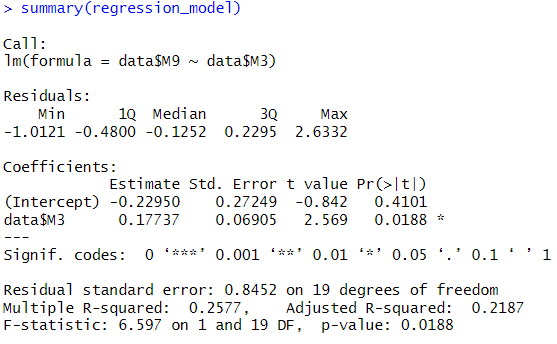
\includegraphics[width=0.6\linewidth]{imagens//questao3/regressaoLinearFinal.png}
    \caption{Modelo de regressão linear final, com as variáveis indicadas pelo stepwise}
    \label{fig:modelo_regressao_linear_final}
\end{figure}


Ao remover as restantes variáveis do modelo, ficando apenas a variável $M3$, o modelo passou de uma regressão linear múltipla para uma regressão linear simples. Agora, para provar a validade do modelo, irão ser feitas as seguintes validações:
\begin{itemize}
    \item Testes globais e Marginais
    \item Análise de Resíduos
    \item Interpretação do $R^2$ % 7\%que é muito pequeno
\end{itemize}


\hfill \break

\subsubsection{Teste Global}
O Teste Global é usado para avaliar conjuntamente a influência de todas as variáveis independentes no modelo da regressão. Para um modelo de regressão linear simples o teste de hipótese é formulado da seguinte maneira:
\hfill \break
\begin{center}
    \(H_0: \, a_1 = 0\) \\
    vs.\\
    \(H_1: \, a_1 \neq 0\)
\end{center}
A hipótese nula \(H_0\) diz que todos os coeficientes \(a_i\) são iguais a zero, indicando que as variáveis independentes não têm efeito significativo na variável dependente. Já a hipótese alternativa \(H_1\) sugere que pelo menos uma variável independente tem um efeito significativo no modelo. Para obter o resultado deste teste precisa-se de ver o p-value que está presente na secção do "F-statistic" na Figura \ref{fig:modelo_regressao_linear_final} caso o p-value lá for menor que o alpha pré-definido (5\%), o que não é o caso, então rejeitar-se-ia a hipótese nula, logo não existe pelo menos um $i$ tal que $a_{i}\ne0$

\subsubsection{Testes Marginais}
 Nos testes marginais, são apenas os testes que se realizaram na análise da regressão, onde se analisa o p-value de cada uma das variáveis independentes, verificando se todas elas têm um p-value ($Pr(>|t|)$) menor que o nível de significância ($\alpha$), caso alguma seja maior, o teste marginal falha. \\
\hfill \break
\begin{center}
    Para cada \(i = 1, 2, 3, ..., n\), o teste individual é formulado da seguinte maneira:
    \newline
    \(H_0: \, a_i = 0\) \\
    vs:\\
    \(H_1: \, a_i \neq 0\)
\end{center}
No modelo de regressão linear final, como só tem uma variável, e como o p-value dessa variável (0.0014) é menor que o nível de significância estabelecido de 5\%, então a hipótese nula é rejeitada, e mais mais uma das validações é realizada.



\subsubsection{Análise de resíduos - Teste de normalidade}
O teste de normalidade pode ser realizado a partir de um teste de Shapiro-Wilk, onde se vai testar a normalidade dos resíduos da regressão, pois um dos pressupostos de uma regressão linear é que os seus resíduos sigam uma distribuição normal. O output do teste realizado pode ser visto na Figura \ref{questao3OutputTesteShapiro}, onde se consegue ver que os resíduos do modelo de regressão linear não seguem uma distribuição normal, logo não passam no teste. O insucesso desse teste pode ser visto a partir do p-value(0.0009263), onde um valor menor que o nível de significância pré-estabelecido (5\%), significa se rejeita a hipótese nula, existindo evidências estatísticas que os resíduos não seguem uma distribuição normal. \\

Teste de Shapiro-Wilk:
\begin{center}
    H0: os resíduos seguem uma distribuição normal
    \newline
    vs:
    \newline
    H1: os resíduos não seguem uma distribuição normal
    \newline
\end{center}

\begin{figure}[!h]
    \centering
    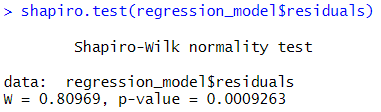
\includegraphics[width=10cm]{imagens/questao3/questao3OutputShapiroTest.png}
    \caption{Output do teste de Shapiro-Wilk para os resíduos da regressão linear}
    \label{questao3OutputTesteShapiro}
\end{figure}

Outra maneira de verificar a normalidade dos resíduos é através de uma representação gráfica da distribuição dos resíduos pela construção de um histograma. No contexto da regressão linear, os resíduos ideais seguiriam uma distribuição normal, resultando em um histograma simétrico com uma forma de um sino, onde os dados se concentram mais no centro, que seria a média. Ao criar um histograma dos resíduos, é possível visualizar a sua distribuição e identificar se ela se assemelha a uma distribuição normal.

\begin{figure}[!h]
    \centering
    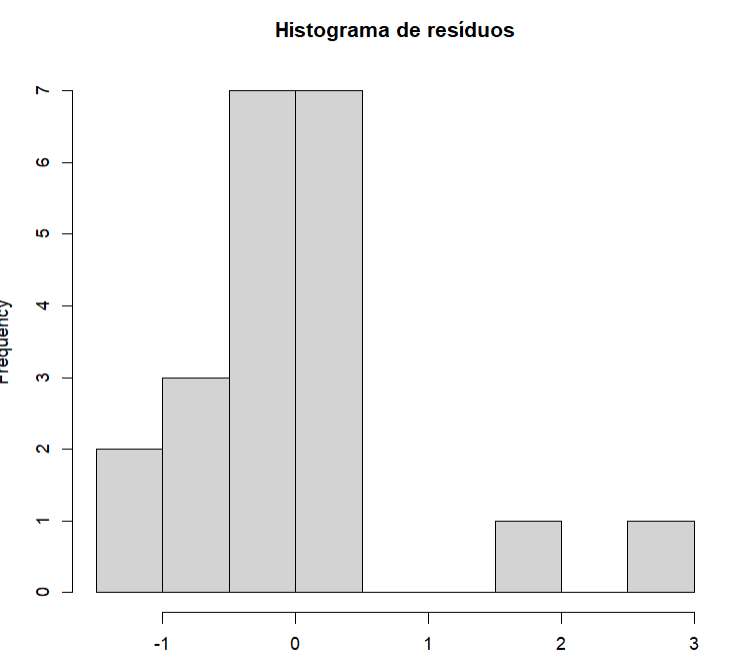
\includegraphics[width=10cm]{imagens/questao3/questao3Histograma.png}
    \caption{Histograma da regressão Linear}
    \label{questao3Histograma}
\end{figure}


Como dá para ver na Figura \ref{questao3Histograma}, mais uma vez foi comprovado que os resíduos da regressão linear não seguem uma distribuição normal, pois o histograma exibe uma assimetria significativa e não apresenta uma forma aproximadamente gaussiana


\subsubsection{Análise de resíduos - Testes de resíduos}
Para os testes de resíduos, pode-se usar um teste de Durbin Wattson, onde se vai testar se os resíduos estão relacionados, se estiverem, então a regressão linear não é válida, pois numa regressão linear, para além dos resíduos terem de seguir uma distribuição normal, eles não devem estar correlacionados. No Output da Figura \ref{questao3OutputTesteDurbinWatson}  dá para ver que o p-value (0.002) é menor que o nível de significância pré-estabelecido (5\%), então a hipótese nula é rejeitada, existindo evidências estatísticas que os resíduos não estão correlacionados, fazendo com que o teste não falhe. \\ \\
Teste de Durbin Wattson:

\begin{center}
    H0: a auto-correlação dos resíduos é igual a 0 
    \newline
    vs:
    \newline
    H1: a auto-correlação dos resíduos é diferente a 0 
    \newline
    \newline
    ou
    \newline
    \newline
    H0:  resíduos estão correlacionados 
    \newline
    vs:
    \newline
    H1: resíduos não estão correlacionados
    \newline
\end{center}

\begin{figure}[!h]
    \centering
    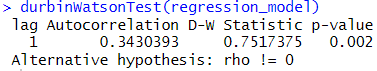
\includegraphics[width=10cm]{imagens/questao3/questao3DurbinWatsonTest.png}
    \caption{Output do teste de Durbin Watson para a correlação dos resíduos}
    \label{questao3OutputTesteDurbinWatson}
\end{figure}



\subsubsection{Interpretação do $R^2$ }
O $R^2$ é uma medida de quão bem o modelo se ajusta aos dados. A interpretação do $R^2$ é essencialmente uma medida da variabilidade explicada pelo modelo em relação à variabilidade total dos dados. Um $R^2$ de 1.0 indica que o modelo explica toda a variabilidade, enquanto um 
$R^2$ de 0 indica que o modelo não explica nada.

Para a análise do $R^2$ da regressão linear proposta anteriormente, precisamos de ir à Figura \ref{fig:modelo_regressao_linear_final}, na secção \textit{"Multiple R-squared: "}, lá é possível ver que o $R^2$ é igual a 0.2577 ou 26\%, que é um valor relativamente pequeno, o que significa que o modelo ajusta-se mal aos dados.

\vspace{2cm}

\textbf{Conclusão:} com o modelo de regressão linear final, pode-se afirmar que a variável $M3$ (número de User Stories abertas) correlaciona com a variável $M9$ (número de testes falhados, por sprint), e ao ter um coeficiente de 0.17737, significa que ao aumento de um valor na variável M4, leva a um aumento de 0.17737 na variável $M9$.

\newpage


\subsection{Questão de Investigação 4}
Para a quarta questão de investigação, decidiu-se investigar os \textbf{fatores que fazer aumentar ou diminuir a métrica do PMD do Class Cohesion (M17)}, para isso, tal como na terceira questão de investigação, será preciso montar um modelo de regressão linear para saber quais variáveis influenciam o valor da variável $M17$.

Para poder montar o modelo de regressão linear, primeiramente observou-se a matriz de correlações realizada na terceira questão de investigação (Figura \ref{questao3matrizDeCorrelacoes}), e a partir daí foi possível observar que as variáveis $M6$, $M7$, $M14$, $M15$ e $M16$ têm uma forte correlação com a variável $M17$, logo são boas candidatas para o modelo de regressão linear.

\begin{itemize}
    \item $M06$ - número de pedidos de alterações rejeitados
    \item $M07$ - número de pedidos de alterações aprovados
    \item $M14$ - Cyclomantic Complexity, número de items menores que 10
    \item $M15$ - Cognitive Complexity, número de items menores que 10
    \item $M16$ - Class Coupling
\end{itemize}

Modelo de regressão linear: \[ M17 = a0 + a1*M06 + a2*M07 + a3*M14 + a4*M15 + a5*M16 + \varepsilon\]

  \begin{figure}[!h]
      \centering
      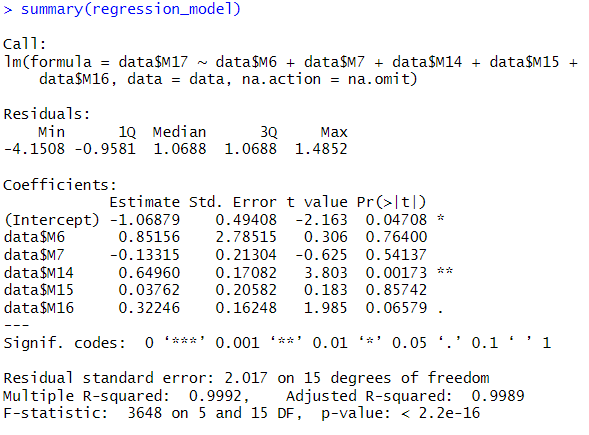
\includegraphics[width=0.6\linewidth]{imagens//questao4/primeiraRegressao.png}
      \caption{Regressão linear múltipla com as variáveis tiradas da matriz de correlações}
      \label{fig:primeiraRegressaoQuartaQuestao}
  \end{figure}

Na Figura \ref{fig:primeiraRegressaoQuartaQuestao} é possível fazer um teste global para saber se o modelo é válido, para isso,  tem que se olhar para a secção F-statistic e verificar se o p-value de lá é menor que o nível de significância estabelecido, como o p-value (0.1514) é maior que o nível de significância estabelecido, isso significa que a hipótese nula não é rejeitada, havendo evidências estatísticas que as variáveis independentes não têm um efeito significativo sobre a variável dependente

Teste Global: 
\begin{center}
        $H0:  a_{1} = a_{2} = ... = a_{i} = 0 $\hspace{0.5cm}
    vs. \hspace{0.5cm}
   $ H1:$  existe pelo menor um i, onde $a_{i} \ne 0$
\end{center}



Para encontrar um modelo de regressão válido, ter-se-ia que descartar variáveis dependentes e executar de novo o modelo de regressão linear sucessivamente até encontrar o modelo mais adequado, para fazer isso utilizou-se uma técnica de seleção de variáveis denominada de \textit{stepwise}.

O método \textit{stepwise} tenta automatizar o processo de seleção das variáveis mais otimizadas para o modelo de regressão linear, considerando critérios como AIC (Akaike Information Criterion) ou BIC (Bayesian Information Criterion). Dessa forma, ao aplicar o \textit{stepwise} o modelo será ajustado consecutivamente, adicionando ou removendo variáveis até encontrar um modelo adequado.


  \begin{figure}
      \centering
      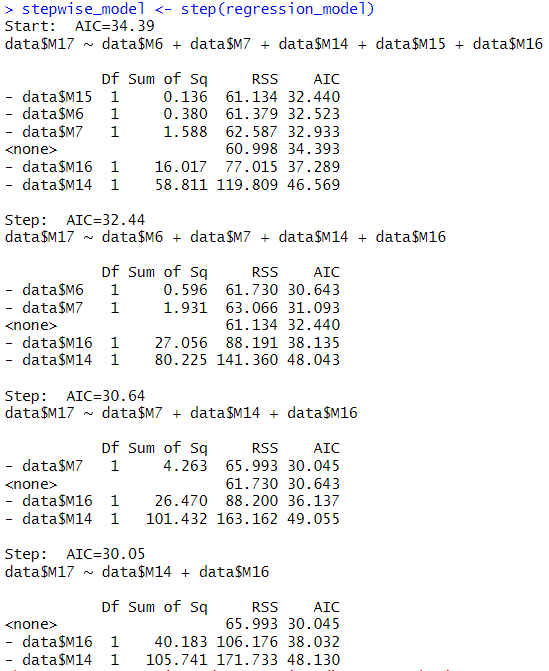
\includegraphics[width=0.6\linewidth]{imagens//questao4/stepwisePergunta4.png}
      \caption{Método stepwise para selecionar as melhores variáveis para o modelo de regressão linear}
      \label{fig:stepwisePergunta4}
  \end{figure}

  Como é possível ver na Figura \ref{fig:stepwiseMethod}, a função iterou até encontrar as melhores variáveis para o modelo de regressão linear, ficando da seguinte forma: 
  
  Modelo de regressão linear: \[ M17 = a0 + a1*M14 + a2*M15 + \varepsilon\]

  \begin{figure}
      \centering
      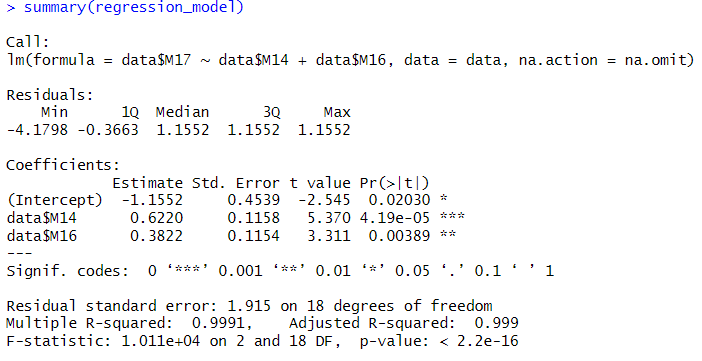
\includegraphics[width=0.6\linewidth]{imagens//questao4/regressaolinearFinalPergunta4.png}
      \caption{Modelo de regressão linear final, com as variáveis indicadas pelo stepwise}
      \label{fig:regressaoLinearFinalPergunta4}
  \end{figure}
Como mostra a Figura \ref{fig:regressaoLinearFinalPergunta4},  todas as variáveis independentes têm um p-value menor que o nível de significância estabelecido de 5\%, existindo evidências estatísticas que todas as variáveis independentes têm impacto sobre a variável dependente.

No entanto, ainda falta comprovar se o modelo de regressão linear é valido com um conjunto de validações, sendo elas:

\begin{itemize}
    \item Testes globais e Marginais
    \item Análise de Resíduos
    \item Interpretação do $R^2$ % 7\%que é muito pequeno
    \item Interpelação dos coeficientes do modelo de regressão
    \item Existência de multicolinariedade entre as variáveis independentes
\end{itemize}


\hfill \break


\subsubsection{Teste Global}
O Teste Global é usado para avaliar conjuntamente a influência de todas as variáveis independentes no modelo da regressão. Para cada \(i = 1, 2, 3, ..., n\), o teste de hipótese é formulado da seguinte maneira:
\hfill \break
\begin{center}
    \(H_0: \, a_1 = a_2 = a_3 = a_4 = 0\) \\
    vs.\\
    \(H_1: \, \text{Existem pelo menos um } i \, \text{tal que} \, a_i \neq 0\)
\end{center}
A hipótese nula \(H_0\) diz que todos os coeficientes \(a_i\) são iguais a zero, indicando que as variáveis independentes não têm efeito significativo na variável dependente. Já a hipótese alternativa \(H_1\) sugere que pelo menos uma variável independente tem um efeito significativo no modelo. Para obter o resultado deste teste precisa-se de ver o p-value que está presente na secção do "F-statistic" na Figura \ref{fig:regressaoLinearFinalPergunta4} caso o p-value lá for menor que o alpha pré-definido (5\%), o que é o caso, então não se rejeita a hipótese nula, havendo evidências que existe pelo menos $i$ tal que $a_{i}\ne0$, que existe pelo menos uma variável independente com um efeito significativo sobre a variável dependente

\subsubsection{Testes Marginais}
 Nos testes marginais, são apenas os testes que se realizaram na análise da regressão, onde se analisa o p-value de cada uma das variáveis independentes, e todas elas têm de ser menores que o nível de significância ($\alpha$), caso alguma seja maior, o teste marginal falha. \\
\begin{center}
    Para cada \(i = 1, 2, 3, ..., n\), o teste individual é formulado da seguinte maneira:
    \newline
    \(H_0: \, a_i = 0\) \\
    vs:\\
    \(H_1: \, a_i \neq 0\)
\end{center}
No modelo de regressão linear final, como o p-value de todas as variáveis independentes são menores que o nível de significância estabelecido de 5\%, então a hipótese nula é rejeitada, e mais mais uma das validações é realizada.


\subsubsection{Análise de resíduos - Teste de normalidade}
O teste de normalidade pode ser realizado a partir de um teste de Shapiro-Wilk, onde se vai testar a normalidade dos resíduos da regressão, pois um dos pressupostos de uma regressão linear é que os seus resíduos sigam uma distribuição normal. O output do teste realizado pode ser visto na Figura \ref{questao4OutputTesteShapiro}, onde se consegue ver que os resíduos do modelo de regressão linear não seguem uma distribuição normal, logo não passam no teste. O insucesso desse teste pode ser visto a partir do p-value($1.621*10^{-5}$), onde um valor menor que o nível de significância pré-estabelecido (5\%), significa se rejeita a hipótese nula, existindo evidências estatísticas que os resíduos não seguem uma distribuição normal. \\

Teste de Shapiro-Wilk:
\begin{center}
    H0: os resíduos seguem uma distribuição normal
    \newline
    vs:
    \newline
    H1: os resíduos não seguem uma distribuição normal
    \newline
\end{center}

\begin{figure}[!h]
    \centering
    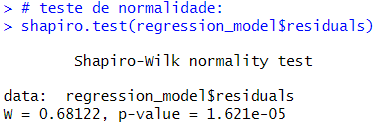
\includegraphics[width=8cm]{imagens/questao4/testeShapiroResiduosPergunta4.png}
    \caption{Output do teste de Shapiro-Wilk para os resíduos da regressão linear}
    \label{questao4OutputTesteShapiro}
\end{figure}

Outra maneira de verificar a normalidade dos resíduos é através de uma representação gráfica da distribuição dos resíduos pela construção de um histograma. No contexto da regressão linear, os resíduos ideais seguiriam uma distribuição normal, resultando em um histograma simétrico com uma forma de um sino, onde os dados se concentram mais no centro, que seria a média. Ao criar um histograma dos resíduos, é possível visualizar a sua distribuição e identificar se ela se assemelha a uma distribuição normal.

\begin{figure}[!h]
    \centering
    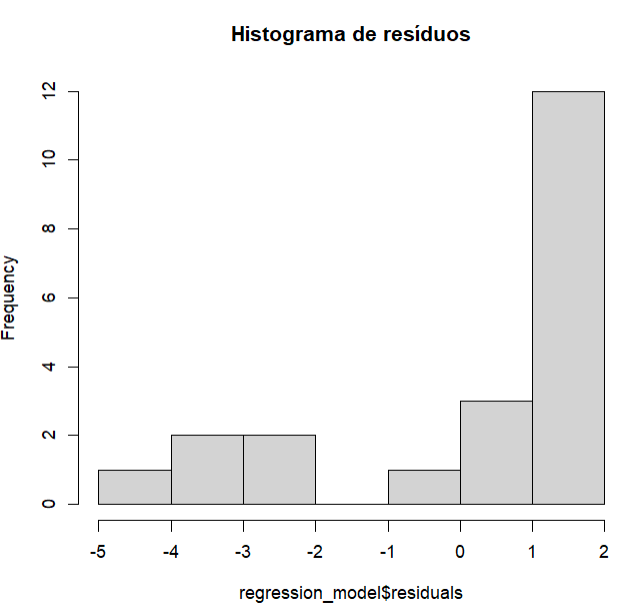
\includegraphics[width=8cm]{imagens/questao4/questao4HistogramaResiduos.png}
    \caption{Histograma da regressão Linear}
    \label{questao4Histograma}
\end{figure}


\subsubsection{Análise de resíduos - Testes de resíduos}
Para os testes de resíduos, pode-se usar um teste de Durbin Wattson, onde se vai testar se os resíduos estão relacionados, se estiverem, então a regressão linear não é válida, pois numa regressão linear, para além dos resíduos terem de seguir uma distribuição normal, eles não devem estar correlacionados. No Output da Figura \ref{questao4OutputTesteDurbinWatson}  dá para ver que o p-value (0.786) é maior que o nível de significância pré-estabelecido (5\%), então a hipótese nula não é rejeitada, existindo evidências estatísticas que os resíduos estão correlacionados, fazendo com que o teste falhe. \\ \\
Teste de Durbin Wattson:

\begin{center}
    H0: a auto-correlação dos resíduos é igual a 0 
    \newline
    vs:
    \newline
    H1: a auto-correlação dos resíduos é diferente a 0 
    \newline
    \newline
    ou
    \newline
    \newline
    H0:  resíduos estão correlacionados 
    \newline
    vs:
    \newline
    H1: resíduos não estão correlacionados
    \newline
\end{center}

\begin{figure}[!h]
    \centering
    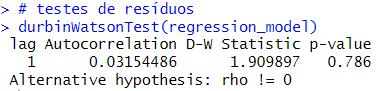
\includegraphics[width=8cm]{imagens/questao4/durbinWatsonTestPergunta4.png}
    \caption{Output do teste de Durbin Watson para a correlação dos resíduos}
    \label{questao4OutputTesteDurbinWatson}
\end{figure}


Como dá para ver na Figura \ref{questao4Histograma}, mais uma vez foi comprovado que os resíduos da regressão linear não seguem uma distribuição normal, pois o histograma exibe uma assimetria significativa e não apresenta uma forma aproximadamente gaussiana




\subsubsection{Interpretação do $R^2$ }
O $R^2$ é uma medida de quão bem o modelo se ajusta aos dados. A interpretação do $R^2$ é essencialmente uma medida da variabilidade explicada pelo modelo em relação à variabilidade total dos dados. Um $R^2$ de 1.0 indica que o modelo explica toda a variabilidade, enquanto um 
$R^2$ de 0 indica que o modelo não explica nada.

Para a análise do $R^2$ da regressão linear proposta anteriormente, precisamos de ir à Figura \ref{fig:regressaoLinearFinalPergunta4}, na secção \textit{"Multiple R-squared: "}, lá é possível ver que o $R^2$ é igual a 0.9991 ou 99\%, que é um valor muito grande, o que significa que o modelo ajusta-se muito bem aos dados.


\subsection{Existência de multicolinariedade entre as variáveis independentes}

A multicolinariedade é a existência de uma forte correlação entre as variáveis independentes de uma regressão linear múltipla, a existência de multicolinariedade pode implicar numa má interpretação dos coeficientes e consequentemente na qualidade da regressão. Para medir a multicolinariedade da regressão linear calculou-se o fator de variação (\textit{VIF}) que nos dá um valor que nos permite avaliar a multicolinariedade das variáveis independentes, onde valores altos referem-se a uma maior multicolinariedade.
Como pode ser visto na Figura \ref{questao4VIF}, as variáveis $M14$ e $M16$ têm um VIF bastante elevado ($268.673$), havendo uma forte correlação entre as duas variáveis, existindo evidências da presença de multicolinariedade na regressão linear.

\begin{figure}[!h]
    \centering
    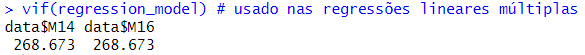
\includegraphics[width=11cm]{imagens/questao4/vif.png}
    \caption{Fator de variação da regressão linear múltipla}
    \label{questao4VIF}
\end{figure}


\vspace{2cm}

\subsection{Clusters}
Para poder observar padrões na regressão linear, pode-se dividi-la em grupos ou clusters, assim, é possível fazer uma visão das relações entre as variáveis independentes e as variáveis dependentes. Para a regressão linear desta questão de investigação, vai-se usar técnicas de clustering dos resíduos, deste modo vai-se agrupar os resíduos semelhantes em clusters específicos, revelando informações importantes sobre a qualidade do modelo.

Para fazer os clusters dos resíduos da regressão linear usou-se um algoritmo denominado de \textit{k-means}, que itera entre atribuir observações aos clusters mais próximos e recalcular os centros dos clusters, até que a atribuição de clusters se estabilize.

Antes de realizar o k-means, é necessário saber quantos clusters são necessários, isso pode ser visto ao interpretar visualmente os dados, ou pelo uso de técnicas como a que se vai usar a seguir, denominada de \textit{método de  Elbow}. A partir desse método foi gerado o gráfico da Figura \ref{fig:ElbowMethod}, e lá é possível ver quantos clusters vão ser precisos a partir da linha vermelha, 3 clusters, que é quando começa a gerar uma curva no gráfico, a linha azul é um valor alternativo para o número de clusters.

\begin{figure}[!h]
    \centering
    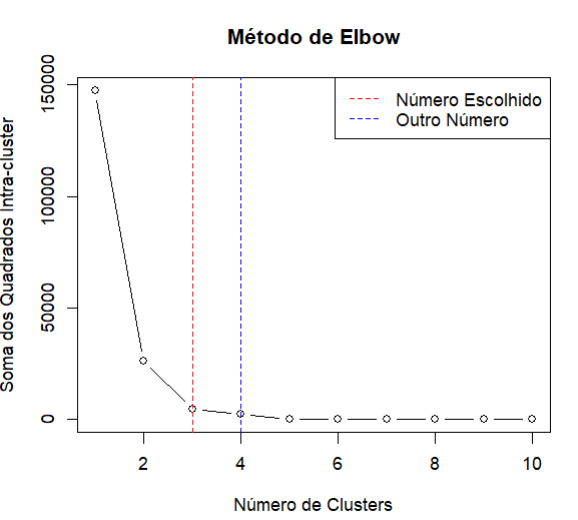
\includegraphics[width=0.6\linewidth]{imagens//questao4/elbowPlot.png}
    \caption{Gráfico do método de Elbow para a seleção do número de clusters }
    \label{fig:ElbowMethod}
\end{figure}

Após se saber que serão precisos no mínimo três clusters, bastou usar apenas a função \textit{k-means} para dividir os resíduos da regressão em clusters, e depois montou-se um boxplot com cada cluster e um gráfico que mostra os dados divididos em cada cluster, a separação é vista a partir da cor de cada ponto.

\begin{figure}[!h]
    \centering
    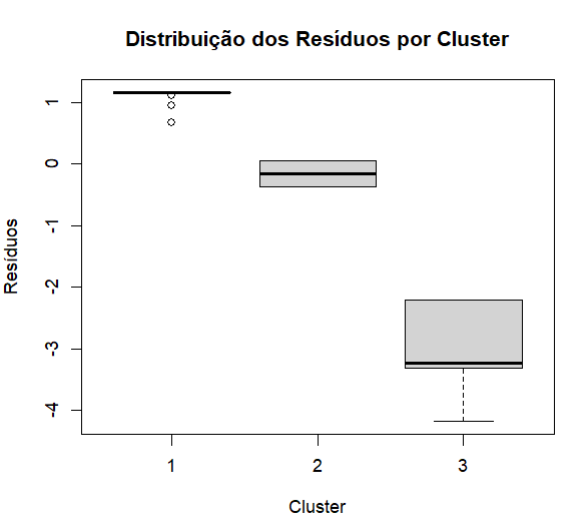
\includegraphics[width=0.4\linewidth]{imagens//questao4/boxplotK-means.png}
    \caption{BoxPlot dos clusters gerados dos resíduos da regressão}
    \label{fig:boxPlotK-means}
\end{figure}


\begin{figure}[!h]
    \centering
    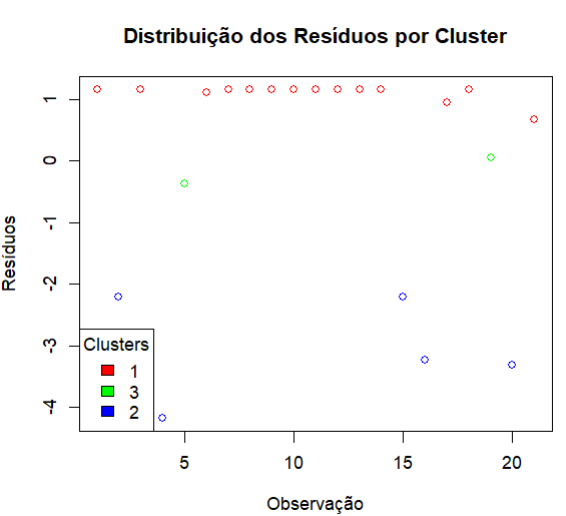
\includegraphics[width=0.4\linewidth]{imagens//questao4/plotClusters.png}
    \caption{Gráfico com a distribuição dos resíduos da regressão linear por cluster}
    \label{fig:plotClusters}
\end{figure}

Como dá para ver na Figura \ref{fig:plotClusters} os pontos entre os clusters encontram-se dispersos, sobretudo no terceiro cluster que só tem dois pontos, e estão muito dispersos, isso pode sugerir que a variabilidade dos resíduos não é fortemente influenciada pela associação a um determinado cluster, no segundo cluster isso também acontece, mas acaba por ser mais fácil de o identificar através da análise do boxplot da Figura \ref{fig:boxPlotK-means}, em que esse cluster apresenta uma caixa maior, logo uma maior variabilidade entre os resíduos do cluster. A partir do boxplot, é possível ver que as caixas dos clusters têm tamanhos bastante diferentes, isso significa que os resíduos não são homogéneos.
\\
Por último, foi calculada a média para cada cluster, apresentando os valores presentes na Figura \ref{fig:mediaClusters},  onde é possível ver que a média dos três cluster é muito próxima de zero, isso significa que os resíduos não apresentam uma tendência significativa, isto é, que se ajustam mal ao modelo.

\begin{figure}[!h]
    \centering
    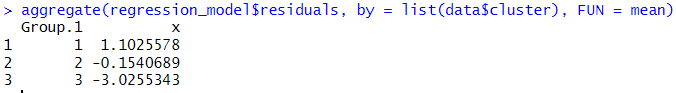
\includegraphics[width=0.6\linewidth]{imagens//questao4/agregateMethod.png}
    \caption{Médias de cada cluster dos resíduos da regressão linear}
    \label{fig:mediaClusters}
\end{figure}

\vspace{1cm}

\textbf{Conclusão:} Com o modelo de regressão linear final, pode-se afirmar que as variáveis $M14$ (Cyclomantic Complexity) e $M16$ (Class Coupling) correlacionam com a variável $M17$ (Class Cohesion). A variável $M14$ ao ter um coeficiente de 0.6220, e a variável $M16$ ao ter um coeficiente de 0.3822, significa que ao aumento de um valor nessas variáveis, leva a um aumento de 0.6220 ou 0.3822 na variável $M9$.

\newpage

% - * - * - * - * - * - * - * - * - * - * - * - * - * - * - * - * - * - *
\section{CONCLUSÕES E TRABALHO FUTURO \label{sec:Conclusions}} 

O objetivo da realização deste projeto foi colocar em pratica todos os tópicos lecionados na unidade curricular de Matemática Computacional II, sendo que os dados para estudo foram retirados do trabalho prático realizado no âmbito da Unidade Curricular de Engenharia de Software II, servindo também para retirar conclusões e complementar a componente estatística desta unidade curricular.

Concluímos que este trabalho nos ajudou a perceber a evolução notória de algumas métricas ao longo de cada recolha. Podemos ainda tirar conclusões sobre se algumas métricas têm alguma influência sob outras o que se revela bastante interessante e importante uma vez que, através dessas conclusões podem ser evitados erros/problemas. Isto foi especialmente importante no que se refere ao desenvolvimento do projeto de Engenharia de Software II, uma vez que nos permitiu acompanhar o crescimento do nosso trabalho, servindo de indicador do nosso próprio progresso.

No entanto, devido ao facto dos dados serem bastante inconstantes, os estudos apresentados ao longo deste relatório podem não ser os mais precisos possíveis. Outra limitação foi o facto de termos mais trabalhos para realizar o que nos fez ficar divididos e não nos focar tanto no neste trabalho. Apesar disto, tomámos decisões e foram adotadas medidas para tornar este relatório o mais completo e preciso possível, mesmo havendo incongruências nos dados, e limitações temporais.

Em relação ao desenvolvimento de trabalhos e relatórios futuros, idealmente seria possível tratar os dados de uma forma mais uniforme, permitindo ter em conta toda a informação e desta forma apresentar resultados mais úteis e precisos. Seria também interessante conseguir avaliar eventuais diferentes métricas.

    



\begin{acknowledgments}
Gostaríamos de agradecer às professoras Eliana Costa e Silva e Maria João Polidoro pelo apoio fundamental durante o trabalho. Suas orientações foram essenciais para a análise estatística, contribuindo significativamente para o desenvolvimento deste projeto.

\end{acknowledgments}

% Bibliografia
%bibliography file "references.bib".
\bibliographystyle{abbrv}
\nocite{overleaf, material}
\bibliography{references.bib}

%\printbibliography %Prints bibliography

\end{document}
%
% ****** End of file aipsamp.tex ******








